\documentclass[a4paper,12pt]{article}
\usepackage[T2A]{fontenc}            % внутренняя кодировка  TeX
\usepackage{amsmath} 
\usepackage{mathtext}
\usepackage{amsfonts}
\usepackage[english,russian]{babel}
\usepackage{graphicx}
\usepackage{textcomp}
\usepackage{geometry}
\geometry{left=3cm}
\geometry{right=1.5cm}
\geometry{top=2cm}
\geometry{bottom=2cm}
\usepackage{tikz}
\usepackage{titling}
\usepackage{indentfirst}
\setlength{\parindent}{1cm}
\usepackage{soul}


\usepackage{enumitem}
\makeatletter
\AddEnumerateCounter{\asbuk}{\russian@alph}{щ}
\makeatother

\pretitle{\begin{flushleft}\Large\textbf}
\title{Декомпозиция линейных автоматов над кольцом вычетов в сдвиговые регистры \protect\footnote{Результаты приведённые в данной работе являются частью докторской диссертации автора, которой руководил профессор Урс Вюрглер (Urs Würgler) из Бернского университета.}}
\posttitle{\end{flushleft}}

\preauthor{\begin{flushleft}}
\author{Арнольд Шойинг (Arnold Scheuing)}
\postauthor{\end{flushleft}}

\predate{\begin{flushleft}}
\date{\textit{\scriptsize{Институт информатики и прикладной математики, Бернский университет, CH-3012 Берн, Швейцария}}}
\postdate{\end{flushleft}}


\begin{document}

\maketitle

\begin{abstract}
	Линейный автомат $\mathfrak{A}$ над факторкольцом $\mathbb{Z}_{n}$, $n \in \mathbb{N}$, в общем случае неразложим на параллельно соединённые сдвиговые регистры. Мы смогли сформулировать необходимые и достаточные условия для такого разложения, используя торию об артиновых локальных кольцах $R$ и $R[x]$-модульной структуре $\mathfrak{A}$.

\end{abstract}

\section{Введение}

Структура конечного, детерминированного линейного автомата (далее КА) интересна не только с точки зрения информатики, но и с точки зрения теории систем. Сфера применений КА, называемых также линейными последовательными схемами (LCS) включает в себя обнаружение и исправление ошибок, генераторы случайных чисел, криптологию (мотивация автора), а также конечномерные линейные системы с постоянными коэффициентами и дискретным или непрерывным временем. До тех пор пока коэффициенты такого автомата или системы являются элементами поля $F$, структура хорошо известна и тщательно изучалась последние двадцать лет \cite{bib4} с помощью линейной алгебры: пространство состояний $E$ автомата $\mathfrak{A}$ --- это конечномерное векторное пространство $E$ над $F$, а функция перехода может быть рассмотрена как эндоморфизм в $E$ или как матрица $A$ над $F$, если базис в $E$ зафиксирован.

Для нахождения более "простого" эквивалентного $\mathfrak{A}$ КА можно использовать взаимооднозначное соответствие между КА, эквивалентными $\mathfrak{A}$, и матрицами, подобными $A$. Есть существенные причины для выбора рациональной канонической формы $A$ как наиболее "простой", потому что она соответствует разложению $A$ на параллельные сдвиговые регистры.

На рисунке \ref{fig1abc} мы показываем три представления КА относительно данного базиса $B$ в $E$. Рисунок \ref{fig1abc}(а) соответствует сдвиговому регистру (его технической реализации) с 3-мерным пространством состояний, каждое из которых обладает компонентами $(s_1, s_2, s_3)$. В теории систем $s_i$ и $a_i$ называются, соответственно, элементами задержки и умножения. Каждый такт элемент из $s_3$ переходит в $s_2$, из $s_2$ --- в $s_1$ и сумма $a_0 s_1 + a_1 s_2 + a_2 s_3$ (в поле $F$) попадает в $s_3$. На рисунке \ref{fig1abc}(б) изображено представление линейной функции $f$ в форме матрицы $3 \times 3$. Эта специальная форма называется сопровождающей матрицей. Если полином $x^3 - a_2 x^2 - a_1 x - a_0$ является несократимым в $F[x]$, тогда КА нельзя разложить. Рисунок \ref{fig1abc}(в) указывает $F[x]$-модуль ранга 3, например, базис $B$ имеет три элемента: $e$, $f(e)$, $f^2(e)$, и
$$
f^3(e) = a_0 e + a_1 f(e) + a_2 f^2(e).
$$

\begin{figure}[h]
	\centering
	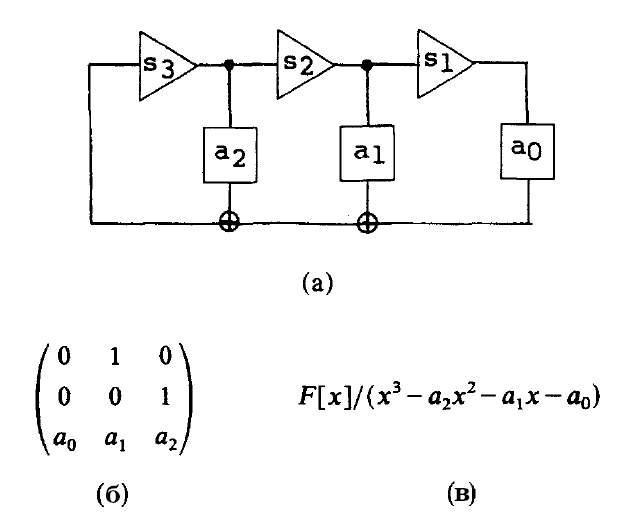
\includegraphics[width=0.5\linewidth]{pictures/fig1abc.png}
	\caption{Соответствующие представления $(a_0, a_1 , a_2 \in F)$. (а) Сдвиговый регистр. (б) Сопровождающая матрица. (в) Циклический F[x]-модуль ранга 3.}
	\label{fig1abc}
\end{figure}

Взаимооднозначное соответствие между этими структурами используется на всём протяжении данной работы: диаграммы КА и сдвиговые регистры для визуализации технической реализации, матрицы для расчётов в примерах, а модули для развития теории.

Известно, что КА с коэффициентами над полем может быть всегда реализован с помощью параллельного соединения сдвиговых регистров \cite{bib9}. Но в применениях, указанных выше, нас также интересуют системы над кольцами $\mathbb{Z} \mod 2^r (r \in \mathbb{N})$. Например, в криптологии процесс автоматизированного шифрования и расшифрования связан с диапазоном значений $2^r$ регистра с $r$ бинарными разрядами.

Хорошее исследование расширения теории линейных систем от полей до колец за последние десять лет можно найти в работе \cite{bib12}. Принцип двойственности для линейных систем над факторкольцами рассматривалась в работах \cite{bib2,bib8}. Представление матричных дробей для линейных систем над коммутативными кольцами также было изучено в работе \cite{bib5}.

В разделе 5 мы приводим пример КА над $\mathbb{Z}_4$, который и не является, и не разложим на сдвиговые регистры. Следовательно, возникает вопрос, при каких условиях КА над $\mathbb{Z}_n$ может быть реализован как параллельное соединение сдвиговых регистров. Похожая проблема изучалась в работах \cite{bib6, bib7}, путём использования биекции $\beta : \mathbb{Z}_{p^r} \approx \prod_{1}^{r}\mathbb{Z}_p$ для декомпозиции КА $\mathfrak{A}$ над $\mathbb{Z}_{p^r}$ в каскад из $r$ автоматов $\mathfrak{A}_i$ над $\mathbb{Z}_p$. Но поскольку $\beta$ не является гомоморфизмом колец, $\mathfrak{A}_i$ соединены с помощью нелинейной логикой без задержек, которая ограничивает дальнейший анализ посредством коммутативной алгебры.

Данная работа состоит из следующих разделов: в разделе 2 мы покажем, что $\mathbb{Z}_{n}$-свободные $\mathbb{Z}_{n}[x]$-модули являются подходящими математическими объектами для изучения структуры КА над полем $\mathbb{Z}_{n}$ (рисунок \ref{fig1abc}). В разделе 3 мы докажем что проблема может быть сведена к КА над $\mathbb{Z}_{p}$ без потери общности; с другой стороны, рекурсивный критерий в последнем разделе предлагает не ограничивать наше внимание на конечных и локальных кольцах $\mathbb{Z}_{p^r}$, а рассматривать более общие (коммутативные) артиновы локальные кольца $R$ (с 1). Следовательно, в разделе 3 мы соберём все необходимые утверждения относительно артиновых локальных колец и модулей над ними. В разделе 4 мы покажем, что наш $R[x]$-модуль всегда имеет \hl{примарное} разложение. Основные результаты находятся в разделах 5 и 6, где мы приводим необходимые и достаточные условия для циклического разложения пространства состояний; другими словами, условия для того, чтобы КА был эквивалентен прямой сумме сдвиговых регистров. Общий случай мы рассматриваем в разделе 5, а специальный с кольцом главных идеалов --- в разделе 6.


\section{Модульная структура конечного автомата}

Начнём с более точного описания конечного автомата (КА).

\paragraph{Определение 2.1}

Конечный детерминированный линейный автомат (без входных или выходных функций) над кольцом $R$ --- это пара $(E,f)$, где пространство состояний $E$ является свободным $R$-модулем конечной размерности (скажем $n$), а функция перехода $f$ --- это линейное отображение из $E$ в $E$. Каждое $e \in E$ является состоянием КА, функция перехода отображает состояние $e$ в новое $f(e)$. Мы можем использовать простую нотацию без начального состояния, потому что нас интересует структура КА в целом.

Множество функций переходов над $E$ --- это кольцо эндоморфизмов $End_R(E) = \{f : E \rightarrow E | f линейна\}$. $End_R(E)$ также является $R$-модулем. Этот факт может быть выражен с помощью гомоморфизма колец на следующей коммутативной диаграмме.

\begin{figure}[h]
	\centering
	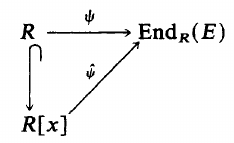
\includegraphics[width=0.25\linewidth]{pictures/diag_1.png}
%	\label{diag_1}
\end{figure}

Для $r \in R$, $\psi(r)$ --- это скалярное произведение для $r$ из $E$. Так как $f$ линейна над $E$, мы можем расширить $\psi$ на $R[x]$ как гомоморфизм колец с помощью задания $\hat{\psi}(x) := f$. Теперь $E$ становится $R[x]$-модулем.

Путём параллельного соединения различных КА над одним и тем же кольцом мы можем построить более крупный автомат. Но ещё больший интерес представляет возможность разложения данного (сложного) автомата на мельчайшие, несократимые части --- сдвиговые регистры.

\paragraph{Определение 2.2}
КА $(E,f)$ над кольцом $R$ называется \textit{сдвиговым регистром}, если $E$ цикличное, как $R[x]$-модуль. Другими словами, если существует такое начальное состояние $e \in E$, что его орбита:
$$
e, f(e), f^2(e), ..., f^{n-1}(e)
$$
охватывает $E$.

Под "<параллельным соединением КА $(E_i, f_i)$"> мы подразумеваем техническую реализацию (см. рисунок \ref{fig2ab}(б)), но оно попросту означает прямую сумму КА $(\bigoplus{E_i}, \bigoplus{f_i})$. Высказывание "<КА реализован как параллельное соединение сдвиговых регистров"> является интуитивным способом выразить то, что $E$ --- это прямая сумма $R[x]$-цикличных $R$-свободных подмодулей.

Для формулировки первой теоремы необходима следующая нотация:

\begin{itemize}
	\item $M_n(R)$ --- множество всех $n \times n$-матриц над $R$,
	\item $GL_n(R)$ --- подмножество всех регулярных матриц из $M_n(R)$,
	\item $M_n(R)/GL_n(R)$ --- множество всех классов подобия матриц ($A \in M_n(R)$ подобна $T^{-1}AT$ для всех $T \in GL_n(R)$),
	\item $Mod_n(Rp[x])$ --- класс всех $R$-свободных $R[x]$-модулей $E$ ранга $n$ (т.е. $dim_R(E) = n$),
	\item $Iso(Mod_n(R[x]))$ --- множество классов изоморфизма таких модулей.
\end{itemize}


\paragraph{Теорема 2.3} Существует биекция:
$$
\chi : M_n(R)/GL_n(R) \rightarrow Iso(Mod_n(R[x]))
$$
\paragraph{Доказательство.}
\hl{Определение $\chi$: Пусть $[A] \in M_n(R)/GL_n(R) ~ и ~ A \in M_n(R)$ --- представители}.
Далее, пусть $E$ --- свободный $R$-модуль ранга $n$. Выберем базис в $E$ и определим $x \cdot e := A \cdot e ~ (\forall e \in E)$. Таким образом $E$ становится $R[x]$-модулем $E_A$. Определим $\chi [A] := [E_A]$ --- класс изоморфизма $E_A$. $\chi$ определено корректно, потому что для подобных матриц $A \sim A'$, модули изоморфны: $E_A \cong E_{A'}$, следовательно, $[E_A] = [E_{A'}]$.

Определение $\chi'$: \hl{Пусть $[F] \in Iso(Mod_n(R[x])) ~ и ~ F \in Mod_n(R[x])$ --- представители}. Выберем $R$-базис в $F$, тогда (линейное) преобразование $x$ может быть выражено с помощью матрицы $A$. Если мы зададим $\chi'[F] := [A]$, то оно также корректно определено и очевидно является обратной функцией к $\chi$.  $\Box$

\section{Артиновы локальные кольца и конечнопорождённые модули}

В первой части этого раздела мы применим китайскую теорему об остатках для упрощения задачи с КА над $\mathbb{Z}_{n}$ до КА над $\mathbb{Z}_{p^r}$ ($p$ --- простое, $r \in \mathbb{N}$).
Мы помним, что кольцо $\mathbb{Z}_{n}$ изоморфно произведению колец $\prod_{i=1}^{m} { {\mathbb{Z}}_{{p_{i}^{r_{i}}}}}$, так как $n$ единственным образом разлагается на простые множители $n = p_1^{t_1} p_2^{t_2} \cdot \cdot \cdot p_m^{t_m}$. Из этого изоморфизма вытекает следующая теорема. 

\paragraph{Теорема 3.1}

Пусть $R_1, R_2, ..., R_m$ --- (коммутативные) кольца (с единицей), $R:=\prod_{i=1}^{m}R_i$, $E$ --- $R$-модуль и определим $E_i := E \otimes R_i$. Тогда кольцо $End_R(E)$ изоморфно $\bigoplus_{i=1}^{m}End_{R_i}(E_i)$.

\paragraph{Доказательство.}
Пусть $f_i := f\otimes1_{E_i} \in End_{R_i}(E_i)$. Мы можем определить гомоморфизм колец $\phi : End_R(E) \rightarrow \bigoplus_{i=1}^{m} End_{R_i} (E_i)$ как $\phi(f) := (f_1, f_2, ..., f_m)$. 

Если $\phi$ --- мономорфизм: для $f \in ker(\phi) \Rightarrow f_i = f \otimes 1_{E_i} = 0 (\forall i) \Rightarrow f(E) \cong \prod_{i}(f(E) \otimes R_i) = 0 \Rightarrow f = $ \hl{(ОПЕЧАТКА: в оригинальной статье формула обрывается).}

Если $\phi$ --- эпиморфизм: мы выбираем произвольное $f_i \in End_{R_i} (E_i)$. Принимая во внимание диаграмму:

\begin{figure}[h]
	\centering
	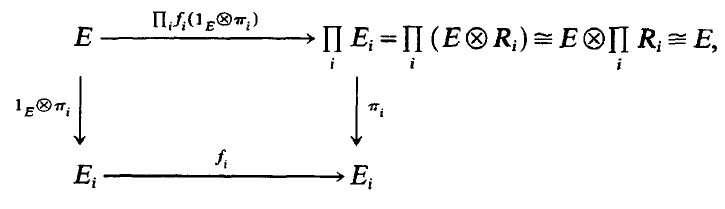
\includegraphics[width=0.5\linewidth]{pictures/diag_2.png}
	%\label{diag_2}
\end{figure}

получаем, что $\phi(\prod_i f_i (1_E \otimes \pi_i)) = (f_1, f_2, ..., f_m)$. $\Box$

\paragraph{Следствие 3.2}
КА над $\mathbb{Z}_n$ может быть всегда реализован с помощью параллельного соединения КА над $\mathbb{Z}_{p^r}$.


\paragraph{Пример 3.3}
КА над $\mathbb{Z}_6$, изображенный на рисунке \ref{fig2ab}(a), изоморфен автомату на рисунке \ref{fig2ab}(b). Соответствующий модуль выглядит следующим образом:
$$
E \cong \mathbb{Z}_6 [x] / (x^3 - 2x^2 - 3x - 4) \cong \mathbb{Z}_2 [x] / (x^3 + x) \oplus \mathbb{Z}_3 [x] / (x^3 + x^2 - 1).
$$

Во второй части данного раздела мы хотим собрать воедино необходимые факты об артиновых локальных кольцах и о модулях над ними.

\begin{figure}[h]
	\centering
	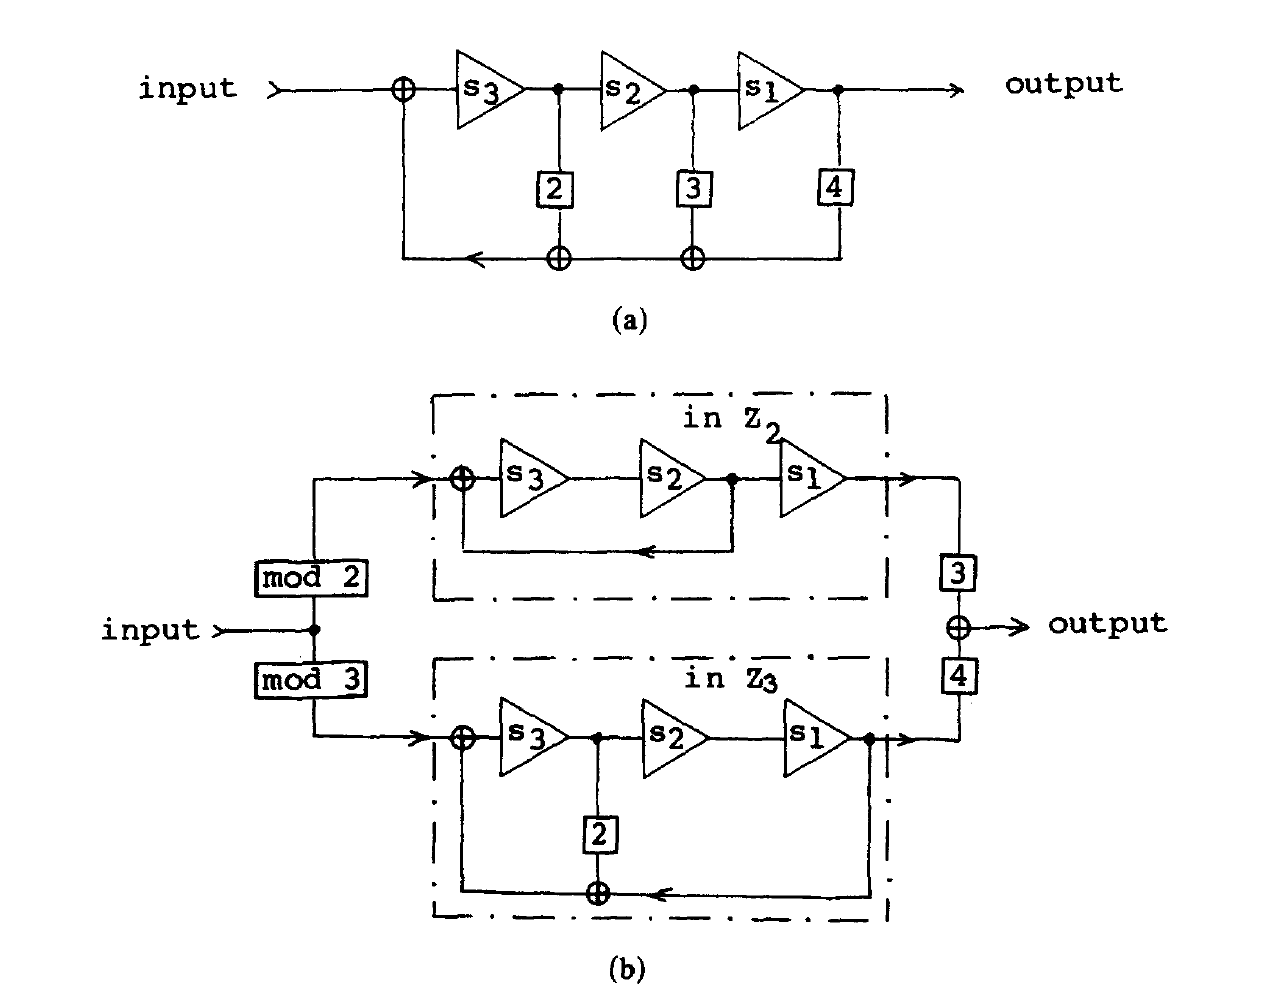
\includegraphics[width=0.75\linewidth]{pictures/fig2ab.png}
	\caption{Эквивалентные КА над $\mathbb{Z}_6$ (со входом и выходом)}
	\label{fig2ab}
\end{figure}

\paragraph{Определение 3.4}
Кольцо $R$ является артиновым, если оно нётерово и имеет размерность 0 (любой простой идеал максимален, см. \cite{bib1}).

Кольцо $R$ является локальным, если оно нётерово и имеет ровно один максимальный идеал $M$. Нотация: $(R,M)$.

\paragraph{Пример 3.5}
$(\mathbb{Z}_{p^r}, (p))$ и $(\mathbb{Z}_{p^r}[x]/(x^S), (p,x))$ --- это артиновы локальные кольца.

\paragraph{Лемма 3.6}
Артиновы локальные кольца $(R,M)$, обладают следующими свойствами:

\renewcommand{\labelenumi}{(\asbuk{enumi})}
\begin{enumerate}
	\item М является единственным простым идеалом;
	\item нильрадикал $Rad(R)$ совпадает с $M$ и сам является нильпотентным; наименьшее $z \in \mathbb{N}$, при котором $M^z = (0)$, называется нильпотентностью $M$;
	\item каждый элемент $R$ либо обратим, либо нильпотентен.
\end{enumerate}

Снэппер (Snapper) \cite{bib11} называет такие кольца "<совершенно простыми кольцами">.

Учитывая важность канонического отображения $\pi : R \rightarrow R / Rad(R)$, мы будем использовать следующую нотацию на всём протяжении работы: $\overline{R} = R / Rad(R)$, \hl{поле остатков}, $\overline{r} = \pi (r) (\forall r \in R), \overline{M[x]} = \pi (M[x]) = 0$.

\paragraph{Примечание 3.7}
В данной работе мы будем рассматривать только конечнопорождённые модули, не повторяя этот факт каждый раз.

Причина, по которой мы не можем следовать такому же разложению, как для автомата над полем $F$ (т.е. как модули над областью главных идеалов $F[x]$), состоит в том, что подмодуль свободного модуля не обязательно является свободным. Но у нас есть следующая фундаментальная теорема.

\paragraph{Теорема 3.8}
(а) В локальном кольце $(S, M)$ все конечнопорождённые модули свободны.

(б) Пусть $(S, M)$ --- артиново локальное кольцо, $F \subset E$ --- оба конечнопорождённые свободные $S$-модули. Тогда $E \cong F \oplus E/F$.

(в) Пусть $(S, M)$ артиново локальное кольцо, $F, G \subset E$ --- три конечнопорождённых свободных $S$-модуля. Тогда $F \cap G$ и $F + G$ являются свободными. 

\paragraph{Доказательство.}
(а) См. \cite{bib10}.

(б) Пусть $\{e_1, ..., e_n\}$ и $\{f_1, ..., f_m\}$ --- базисы в $E$ и $F$, соответственно. Поскольку $F \cap E \Rightarrow f_1 = \sum \phi_i e_i$ и поскольку $\{f_1, ..., f_m\}$ линейно независимы, как минимум один из $\phi_i$ должен быть обратим (см. лемму 3.6). Без потери общности, обратимый $\phi_i$ подразумевает $e_1 = (\phi_1^{-1})(f_1 - \sum_{i < 1} \phi_i e_i)$. Поэтому $\{f_1, e_2, ..., e_n\}$ --- это базис в $E$. По индукции получаем, что $\{f_1, f_2, ..., f_m, e_{m+1}, ..., e_n\}$ является базисом в $E$, следовательно, $E \cong F \oplus L_R (e_{m+1}, ..., e_n)$.

(в) $G \rightarrow F \oplus E/F$ и оба слагаемых свободные (см. часть (б)). Пусть $\{g_1,...,g_p\}$ --- базис в $G$, а $\{f_1, f_2, ..., f_m, e_{m+1}, ..., e_n\}$ --- базис в $E =  F \oplus E/F$. Поскольку $g_i \in E$, мы можем заключить аналогично части (б), что $\{g_1, ..., g_q, f_{q+1}, ..., f_m, g_{q+1}, ..., g_p, e_{n-m-p+q}, ..., e_n\}$ является базисом в $E$. Следовательно, $F \cap G = L_S(g_1, ..., g_q)$ и $F + G = L_S(g_1, ..., g_p, f_{q+1}, ..., f_m)$ свободны. $\Box$ \\

Напомним, что для несократимого полинома $\alpha \in R[x]$, \hl{отображение} $\bar{\alpha} \in \bar{R}[x]$ не обязательно будет несократимым. Если оно является таковым, то мы называем $\alpha$ фундаментально несократимым.


\paragraph{Лемма 3.9}
Вот некоторые важные типы идеалов в $R[x]$ для артинова локального $(R, M)$:

\renewcommand{\labelenumi}{(\asbuk{enumi})}
\begin{enumerate}
	\item $M[x] := \{\sum_i r_i x^i \in R[x] | r_i \in M \} \subset R[x]$ является единственным \hl{нулевым} простым идеалом в $R[x]$;
	\item Все ненулевые простые идеалы имеют вид $M[x] + (\alpha)$, где $\alpha \in R[x]$ приведённый и фундаментально несократимый. Поскольку $\bar{R}$ поле, эти идеалы также являются максимальными;
	\item Ненулевой идеал в $R[x]$ представим в виде $N + (\beta)$, где $\beta$ --- приведённый многочлен и $N \subset M[x]$. Порождающие $N$ могут быть всегда выбраны так, что их степень меньше, чем $\beta$/.
\end{enumerate}

Доказательство очевидно; подробности можно найти в работе \cite{bib11}.

\pagebreak

\begin{thebibliography}{99}
	
	\bibitem{bib1}
	M.F. Atiyah and I.G. MacDonald,
	Introduction to Commutative Algebra
	(Addison-Wesley, Reading, MA, 1969).
	
	\bibitem{bib2}
	W.S. Ching and B.F. Wyman,
	Duality and the regulation problem for linear systems over commutative rings,
	J. Comput. System Sci. 14 (1977) 360-368.

	\bibitem{bib3}	
	T. Hungefford,
	Algebra
	(Holt, Rinehart \& Winston, New York, 1974).
	
	\bibitem{bib4}	
	R.E. Kalman, P.L. Falb and M.A. Arbib,
	Topics in Mathematical System Theory
	(McGraw-Hill, New York, 1969).
	
	\bibitem{bib5}
	P. Khargonekar, On Matrix Fraction Representation for Linear Systems over Commutative Rings
	(Center of Math. System Theory, Univ. of Florida, 1980).
	
	\bibitem{bib6}	
	M. Magidin and A. Gill,
	Decomposition of linear sequential circuits over residue rings,
	J. Franklin Inst. 294 (1972) 167-180.
	
	\bibitem{bib7}	
	M. Magidin and A. Gill,
	Singular shift registers over residue class rings,
	Math. Systems Theory 9(4) (1976) 345-358.
	
	\bibitem{bib8}	
	G. Nandi and C. Nolte,
	Duality for systems over rings,
	Inform. Control 50. (1981) 128-132.
	
	\bibitem{bib9}	
	B. Reusch,
	Lineare Automaten
	(Bibliographisches Institut, Mannheim, 1969).
	
	\bibitem{bib10}	
	J.R. Silvester,
	Introduction to Algebraic K-theory
	(Chapman \& Hall, London, 1981).
	
	\bibitem{bib11}	
	E. Snapper,
	Completely primary rings,
	Ann. of Math. 52 (1950) 666-693.
	
	\bibitem{bib12}	
	E.D. Sontag,
	Linear systems over commutative rings, Ricerche Automat.
	7(1) (1976) 1-34.
	
	\bibitem{bib13}
	B.L. van der Waerden,
	Algebra 2
	(Springer, Berlin, 1967).
	
\end{thebibliography}


\end{document}